\section{Control System}

A well-designed control system is integral for the segway to balance, compensate for any disturbances, and achieve precise control by continuously monitoring quantitative specifications such as its tilt and adjusting the motor output to maintain stability. This will all need to be integrated with the rest of the subsystems as it has the potential to act as the foundation for the segway. Control systems are typically incorporated with a feedback loop, such as a PID (Proportional-Integral-Derivative) system, to dynamically respond to deviations and ensure stable operation.

\subsection{System Requirements and Constraints}

When it comes to thinking about system requirements, it’s important to be mindful of things like operating voltage / power consumption, accuracy of the controller determined by properties such as weight, weight distribution, torque of the motors and inertia of the entire design.

One of the challenges faced was using the correct pins from the ESP32 as they had different specificities (referring to GPIO pins). Furthermore, being limited via the power of the battery meant that the speed and output power of the motors are limited to allow for enough voltage and current to all the other components. One of the ways the effect of this was minimised, was by adjusting the potentiometer values on the A4998 motor drivers to allow for a high voltage without compromising too much on current. 

\newpage

\subsection{Design Approach}
\begin{wrapfigure}{l}{0.3\textwidth}
    \centerline{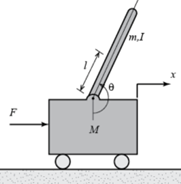
\includegraphics[width=0.28\textwidth]{images/balance.png}}
    \caption{Inverted Pendulum}
    \label{fig:balance}
\end{wrapfigure}
The concept of a self-balancing Segway is derived heavily from the theory of an inverted pendulum. The primary aim of the control system is to balance this inverted pendulum to keep it in an upright pose by applying a force to the base of the segway, via torque produced by the wheels. This is clearly visualised below.


\vspace{2mm}

The inverted pendulum system was stabilised using a proportional-integral-derivative (PID) control approach. A response proportionate to the discrepancy between the desired and actual positions of the pendulum is provided by the proportional term. While the derivative term projects future errors based on the error's rate of change, the integral term integrates the error through time to eliminate steady-state errors. The response of the control system can be enhanced by varying the weights given to each component otherwise known as tuning the PID values.

\begin{figure}
    \centerline{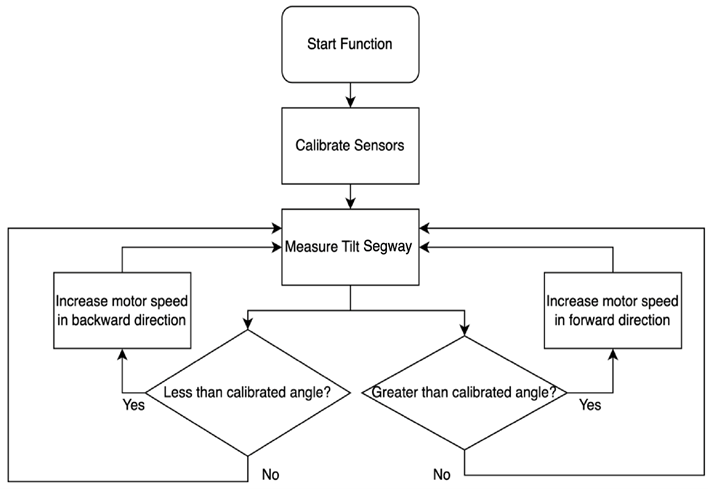
\includegraphics[width=0.8\textwidth]{images/control-flow.png}}
    \caption{Control flow diagram}
\end{figure}
Before diving into building a PID controller, the idea of just a P controller working would allow for easy implementation and design. This flowchart represents a controller that provides a simple reaction by increasing and decreasing the speed of the motor wheels to account for the changes in tilt. This was the original designed controller but proved to have many issues including a slow reaction speed to impulse responses, inaccuracies, and imprecise responses when subject to subtle perturbations.  

\begin{figure}
    \centerline{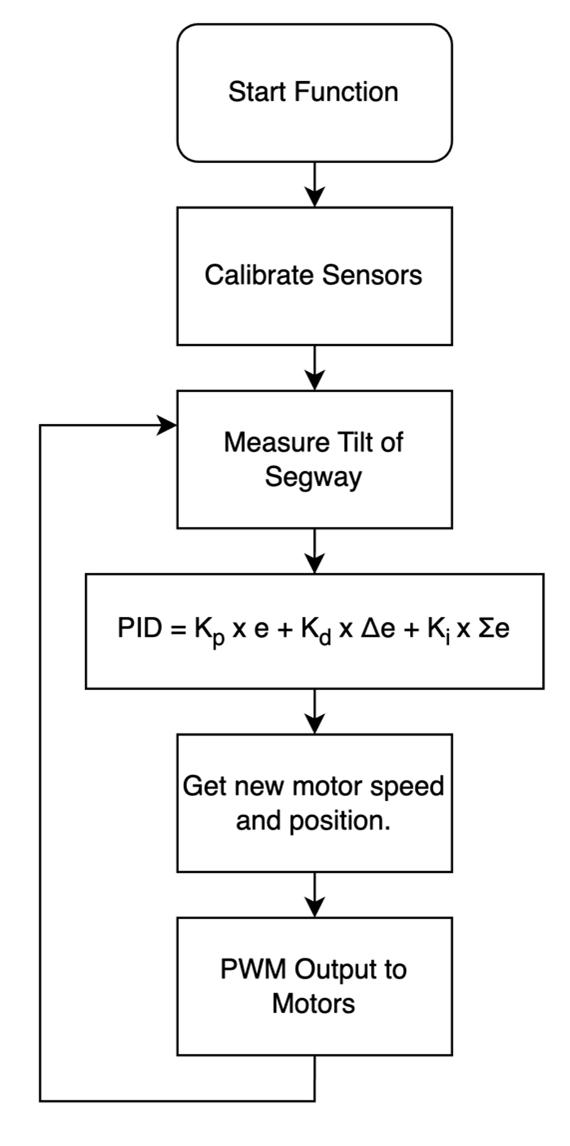
\includegraphics[width=0.28\textwidth]{images/pid-flow.png}}
    \caption{PID controller flow diagram}
\end{figure}
This led to building a PID controller code to consider error. This will allow for improved stability, by eliminating steady state errors that compound over time, reducing overshoot, reducing latency, and increasing robustness of the system.

The code calculates the error by subtracting the target angle from the current angle. It then performs the PID control calculations, which involves multiplying the error by the proportional gain (Kp), the integral gain (Ki), and the derivative gain (Kd), respectively. The integral term and previous error are also updated accordingly.

Adjusting motor speeds based on the PID output, adjusts the speeds of the two stepper motors. If the output is above a certain threshold, the motors rotate in opposite directions to balance the pendulum. If the output is below the threshold, the motors stop.

The calibrateMPU6050() function collects calibration data from the accelerometer and calculates calibration offsets for each axis. These offsets are then subtracted from the raw accelerometer readings to obtain accurate tilt angles.

This in turn would theoretically make the control system self-correcting and thus successfully balance the segway.

\newpage
\subsection{Simulation}

With this design in mind, it would help to build and test a control system using Simulink through MATLAB for further testing and understanding. 

\begin{figure}
    \centerline{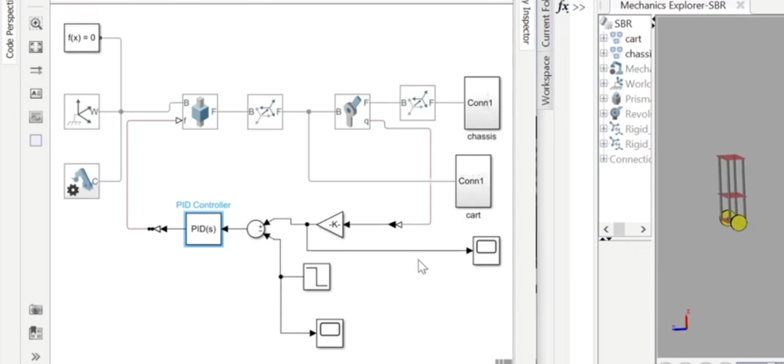
\includegraphics[width=\textwidth]{images/simulink-diagram.png}}
    \caption{Simulink model of PID controller \cite{ref:balance_sim}}
\end{figure}

Using this it is easy to simulate what effect, different values of PID will have on the system. 

The desired goal is to reach a system that has very small oscillations and is \\
ultimately asymptotically stable as demonstrated in figure \ref{fig:simulation-result}.

\begin{wrapfigure}{l}{0.3\textwidth}
    \centerline{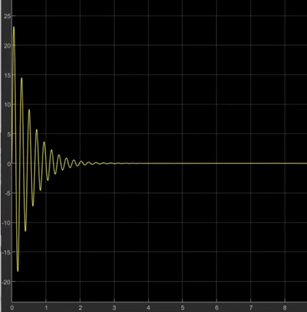
\includegraphics[width=0.28\textwidth]{images/simulation-result.png}}
    \caption{Simulink simulation result}
    \label{fig:simulation-result}
\end{wrapfigure}

By experimenting with the simulation, it became apparent that increasing the P, I, or D terms has the following effects on the overall system:

Increasing the proportional gain (P) amplifies the response of the controller to the error signal. In essence, it makes the controller more sensitive, leading to a stronger corrective action to reduce the error, faster initial response, and potentially higher overshoot.

Increasing the integral gain (I) increases the contribution of accumulated error over time to the control signal, eliminating steady-state errors by continuously adjusting the control output. This would allow the controller to better handle constant or slowly changing errors, improving the system's ability to track and maintain the desired value. However, too high of a value can cause overshoot, oscillations, and instability if not moderated.

Increasing the derivative gain (D) amplifies the contribution of the rate of change of the error to the control signal. It helps the controller anticipate and react to changes in the error signal providing faster response to sudden changes in the error, again, reducing overshoot and damping oscillations.

To summarise, finding the right balance and tuning these gains is crucial for achieving stable and efficient control. To find the true PID values, it would be wise to keep varying the gain values on the finished rover.

Writing the code for it to balance proved to be trivial after installing all relevant libraries and building the simulation on Simulink. Initially, the primary goal of the control system is to get it to balance and that is what is found in the appendix.

\subsection{Movement}

To enable movement while keeping the inverted pendulum upright, one approach is to gradually accelerate the wheel in the desired direction. However, maintaining a constant speed without toppling the pendulum is challenging due to the need for precise torque when starting and stopping. 

When the pendulum is tilted, a force acts on the wheels, requiring an opposing force for balance. To address this, a perturbation method can be employed. By temporarily adjusting the balancing angles obtained during calibration, forward or backward movement can be initiated, followed by a return to the balancing position. Continuous repetition or adjusting the delay allows for consistent movement.

For left and right motion, a function can be implemented to rotate the pendulum quickly. By carefully controlling the movement of both motors independent of the balancing axis, tilting can be minimized. The pendulum can then be returned to a balanced state.

Implementing these strategies enables movement while maintaining the upright position of the inverted pendulum. This is the next step to successfully implement this. 

Sensor integration of the MPU6050 was limited to the nearest 0.5 to act as a filter ensuring the that the smallest perturbations, in which case, may just be noise has no effect on the motors. This allowed the segway to stay relatively still when balancing. After adjusting the potentiometer values on the A4998, it was tuned to allow them to draw the same the voltage and current. This will enhance the segway’s stability property as it ensures that both motors will provide the same torque for forward and backward manoeuvrability. 

Challenges were encountered during calibration, including finding the right balance between responsiveness and stability. Strategies such as trial and error, iterative testing, and observation of the system's behaviour were employed to overcome these challenges. The calibration process ensured that the control system parameters were optimized by minimizing oscillations, preventing overshoot, and maintaining a steady state.

The calibration results demonstrated the impact of the chosen gains and thresholds on the robot's balancing performance. Through careful adjustment, the control system achieved improved stability and accuracy. Evidence of calibration results, such as graphs showing the system's response to disturbances, can be presented to showcase the effectiveness of the calibration process. Regular monitoring and fine-tuning of the control system parameters ensure continued optimal performance and adaptability to varying environments.

\subsection{Testing}

The efficiency of the control system was tested by rigorous testing processes, demonstrating the robot's capacity to balance on two wheels. While limitations were discovered in response to rapid changes or external forces, these difficulties can be addressed through enhancements to the control algorithm and varying chassis height. Calibration was critical in optimising control system characteristics, with evidence showing that modified gains and thresholds had a direct impact on balancing performance. Iterative modifications to PID values and empirical testing were used to overcome problems during calibration. The table can be seen in figure \ref{tbl:pid-iterations} below.
\begin{figure}
    \centering
    \begin{tabular}{ |c|c|c|c|}
        \hline
            \textbf{Iteration}   &   \textbf{kP}  &   \textbf{kI}  &   \textbf{kD}  \\
            \hline
            1	&   1.00	&   0.00    &   0.00 \\
            \hline
            2	&   1.50	&   0.01    &   0.00 \\
            \hline
            3	&   1.50	&   0.00    &   0.01 \\
            \hline
            4	&   1.50	&   0.20    &   0.20 \\
            \hline
            5	&   1.80	&   0.25    &   0.20 \\
            \hline
            6	&   1.90	&   0.25    &   0.35 \\
            \hline
            7	&   2.10	&   0.47    &   0.30 \\
            \hline
            8	&   2.50	&   0.50    &   0.40 \\
            \hline
            9   &   2.80	&   0.45    &   0.45 \\
            \hline
            10  &	3.00    &   0.57    &   0.50 \\
            \hline
            11  &	4.50    &   0.43    &   0.35 \\
            \hline
            12  &	4.80    &   0.45    &   0.30 \\
            \hline
            13  &	4.90    &   0.80    &   0.20 \\
            \hline
            14  &	4.98    &   0.81    &   0.26 \\
            \hline
        \end{tabular}
    \caption{PID Iterations}
\label{tbl:pid-iterations}
\end{figure}
The inclusion of the control system will allow for the segway to balance freely and precisely on the terrain. However, to perfect the control system, it is important to lighten the load on the chassis to allow for a more suitable amount of torque, fully build in the movement functions as mentioned above, utilise both cores on the ESP32 board to ensure that there are no clock delays between the sensor and motor signals and use filters to prevent high frequency oscillations within the system.
